\documentclass[8pt]{beamer}
% Add references to notes
\makeatletter\defbeameroption{show only notes}[]{\beamer@notestrue\beamer@notesnormalsfalse}

% Originally from https://kbroman.org/blog/2013/10/07/better-looking-latexbeamer-slides/
\usetheme{default}
\hypersetup{pdfpagemode=UseNone} % hides bookmarks on initial view
\beamertemplatenavigationsymbolsempty % removes navigation buttons clashing with the defined slide numbers

\setbeamertemplate{sections/subsections in toc}[sections numbered] % replaces bullets in toc with numbers
\setbeamertemplate{bibliography item}{\insertbiblabel} % Numbered bibliography
\setbeamertemplate{itemize subitem}{{\textendash}} % changes bullets to \textendash
% Make bullets/nums smaller
\setbeamerfont{itemize/enumerate subbody}{size=\footnotesize}
\setbeamerfont{itemize/enumerate subitem}{size=\footnotesize}
% Slide number
 \setbeamertemplate{footline}{%
   \raisebox{5pt}{\makebox[\paperwidth]{\hfill\makebox[20pt]{\color{gray}
         \scriptsize\insertframenumber}}}\hspace*{5pt}}

\definecolor{foreground}{RGB}{255,255,255}
\definecolor{background}{RGB}{24,24,24}
\definecolor{title}{RGB}{107,174,214}
\definecolor{gray}{RGB}{155,155,155}
\definecolor{subtitle}{RGB}{102,255,204}
\definecolor{hilight}{RGB}{102,255,204}
\definecolor{vhilight}{RGB}{255,111,207}

\setbeamercolor{titlelike}{fg=title}
\setbeamercolor{subtitle}{fg=subtitle}
\setbeamercolor{institute}{fg=gray}
\setbeamercolor{normal text}{fg=foreground,bg=background}
\setbeamercolor{item}{fg=foreground} % color of bullets
\setbeamercolor{subitem}{fg=gray}
\setbeamercolor{itemize/enumerate subbody}{fg=gray}
\setbeamercolor{section in toc}{fg=foreground}
\setbeamercolor{subsection in toc}{fg=gray}


\usepackage{amsmath} % for more symbols and mafs
\usepackage{hyperref} % for links
\usepackage{fancyvrb}
\usepackage{hyperref}

\usepackage{array}
\newcolumntype{M}{>{\centering\arraybackslash}m{2.2cm}}
\newcolumntype{R}{>{\centering\arraybackslash}m{1.5cm}}

\usepackage{caption}
\captionsetup{justification=raggedleft} % right aligns multiline captions

\graphicspath{{../images/}}

\usepackage[backend=biber, sorting=none]{biblatex}
\addbibresource{../bib.bib}

\usepackage{xepersian} % must be the last package
\settextfont{XB Roya}
\setlatintextfont{Vazir}
\setdigitfont{XB Roya}
\setmonofont{Iosevka}
\usefonttheme{serif} % (Required for Persian)

\makeatletter
% Originally from http://qa.parsilatex.com/14100
% -----
% BEGIN List fix
% -----
\expandafter\let\csname beamer@@tmpop@itemize item@default\endcsname\relax
\expandafter\let\csname beamer@@tmpop@itemize subitem@default\endcsname\relax
\expandafter\let\csname beamer@@tmpop@itemize subsubitem@default\endcsname\relax

\defbeamertemplate*{itemize item}{default}{\scriptsize\raise1.25pt\hbox{\donotcoloroutermaths$\blacktriangleleft$}}
\defbeamertemplate*{itemize subitem}{default}{\tiny\raise1.5pt\hbox{\donotcoloroutermaths$\blacktriangleleft$}}
\defbeamertemplate*{itemize subsubitem}{default}{\tiny\raise1.5pt\hbox{\donotcoloroutermaths$\blacktriangleleft$}}

\patchcmd{\@listi}{\leftmargin}{\rightmargin}{}{}
\let\@listI\@listi
\patchcmd{\@listii}{\leftmargin}{\rightmargin}{}{}
\patchcmd{\@listiii}{\leftmargin}{\rightmargin}{}{}
\patchcmd{\beamer@enum@}{\raggedright}{\raggedleft}{}{}
\patchcmd{\@@description}{\raggedright}{\raggedleft}{}{}
\patchcmd{\@@description}{\leftmargin}{\rightmargin}{}{}

\renewcommand{\itemize}[1][]{
  \beamer@ifempty{#1}{}{\def\beamer@defaultospec{#1}}
  \ifnum \@itemdepth >2\relax\@toodeep\else
    \advance\@itemdepth\@ne
    \beamer@computepref\@itemdepth% sets \beameritemnestingprefix
    \usebeamerfont{itemize/enumerate \beameritemnestingprefix body}%
    \usebeamercolor[fg]{itemize/enumerate \beameritemnestingprefix body}%
    \usebeamertemplate{itemize/enumerate \beameritemnestingprefix body begin}%
    \list{\usebeamertemplate{itemize \beameritemnestingprefix item}}{\def\makelabel##1{{
      \hss\llap{{
        \usebeamerfont*{itemize \beameritemnestingprefix item}
        \usebeamercolor[fg]{itemize \beameritemnestingprefix item}##1}}
      }}
    }
  \fi
  \beamer@cramped
  \raggedleft
  \beamer@firstlineitemizeunskip
}
% -----
% END List fix
% -----
% BEGIN TOC fix
% -----
\expandafter\let\csname beamer@@tmpop@subsection in toc@default\endcsname\relax
\expandafter\let\csname beamer@@tmpop@subsubsection in toc@default\endcsname\relax
\defbeamertemplate*{subsection in toc}{default}
{\leavevmode\rightskip=1.5em\inserttocsubsection\par}

\defbeamertemplate*{subsubsection in toc}{default}
{\leavevmode\normalsize\usebeamerfont{subsection in toc}\rightskip=3em
  \usebeamerfont{subsubsection in toc}\inserttocsubsubsection\par}
% -----
% END TOC fix
% -----
\makeatother

\raggedleft % right aligns for Persian texts


\author{محمدیاسین داوده}
\title{لینوکس}
\subtitle{هرآنچه لازم است بدانید}
\date{\today}

\newcommand{\start}[1][نقشه راه]{
  \frame{\maketitle}
  \begin{frame}{#1}\tableofcontents\end{frame}
}

\newcommand{\bib}{
  \begin{LTR}
    \printbibliography[heading=none]
  \end{LTR}
}

\newcommand{\refs}{
  \section{مراجع}
  \begin{frame}[allowframebreaks]{مراجع}
    \bib
  \end{frame}
  \note{\bib}
}

\newcommand{\subt}[1]{{\footnotesize\color{subtitle}{#1}}}

\newcommand{\divider}[1]{\frame{\Huge{#1}}}

\newcommand{\subdivider}[1]{\frame{\color{hilight}\huge{#1}}}

\newcommand{\alongside}{\and\\\small\smallskip}

\newcommand{\singleton}[2][]{
  \begin{frame}{#1}
    \centering
    #2
  \end{frame}
}

\newcommand{\includetwins}[3][\textwidth]{
  \includegraphics[width=.49#1]{#2}
  \includegraphics[width=.49#1]{#3}
}
% -----
% BEGIN Code (minted)
% -----
\newenvironment{code*}[2][]{
  \VerbatimEnvironment
  \begin{LTR}
    \begin{minted}[#1, linenos, mathescape]{#2}%
    }{
    \end{minted}
  \end{LTR}
}

\newcommand{\codecaption}[1][]{\captionsetup{type=listings}\captionof{listing}{#1}}

\AtBeginEnvironment{minted}{\renewcommand{\fcolorbox}[4][]{#4}} % Disable syntax error red boxes
% -----
% END Code (minted)
% -----


\begin{document}
\start

% صفحه ۱

\begin{frame}{نصب و راه اندازی ~\cite{Debian_book}}
  برای نصب و راه اندازی می‌توان به راحتی از نصاب دبیین استفاده کرد که این امر مراحل نصب را ماژولار می‌کند که باعث می‌شود شخصی سازی کردن مراحل نصب آسان‌تر شود.\\
 \textbf{سیستم مورد نیاز برای نصب بدون محیط گرافیکی:}
 \begin{itemize}
   \item ۱۲۸ مگابایت رم
   \item ۲ گیگابایت حافظه
\end{itemize}
\textbf{سیستم مورد نیاز برای نصب همراه با محیط گرافیکی}
\begin{itemize}
  \item ۱ گیگابایت رم
  \item ۱۰ گیگابایت حافظه
\end{itemize}
\end{frame}

% صفحه ۲

\section{متدهای مختلف نصب}
\begin{frame}{متدهای مختلف نصب}
  دبین را از طریق راه‌های مختلفی می‌توان نصب کرد. ابتدا باید بررسی کرد که BIOS سیستم شما از چه راه‌هایی به شما دسترسی می‌دهد.\\
 به وسیله راه‌های زیر می‌توانید آن را بوت کنید:
\begin{enumerate}
  \item CD-ROM/DVD-ROM
  \item USB Storage
  \item شبکه
\end{enumerate}
\end{frame}
\note{
  Note: BIOS(Basic Input / Output System)
نرم افزاری که در مادربرد است و زمانی که کامپیوتر بوت می‌شود اجرا می‌شود، تا سیستم عامل را به وسیله یک بوت لودر منطبق مانند گراب اجرا می‌کند.
}

% صفحه ۳

\subsection{نصب از طریق CD/DVD}
\begin{frame}{نصب از طریق ایمیج موجود در CD}
  یکی از متداول ترین راه‌های نصب از روی CD است.
کامپیوتر از روی CD بوت می‌شود و مراحل نصب شروع می‌شود. درون CD یک فایل ایمیج ISO قرار دارد که اگر سیستم شما به اینترنت دسترسی ندارد تمام نرم‌افزارهای پایه مورد نیاز به وسیله همان فایل ISO درون CD نصب می‌شود.
نوعی دیگر از ایمیج‌ها mini.iso  است که پایه ترین پکیج‌های مورد نیاز را دارد و بقیه پکیج‌ها باید دانلود شوند.
\begin{figure}
    \centering
    
\includegraphics[width=0.3\textwidth]{debian-logo}
    \caption{لوگو دبیین~\cite{wp:deb_live}}
\end{figure}
\end{frame}

% صفحه ۴

\subsection{نصب از طریق USB}
\begin{frame}{نصب از طریق ایمیج موجود در حافظه USB}
  اغلب رایانه‌ها دارای قابلیت اتصال حافظه‌ی خارجی از طریق پورت USB هستند و این امر کمک می‌کند تا به وسیله یه کارت حافظه قابل حمل که با درگاه‌های USB سازگار است، دبیین و حتی دیگر توزیع‌های لینوکس را نصب کنید.
\begin{figure}
  \centering
  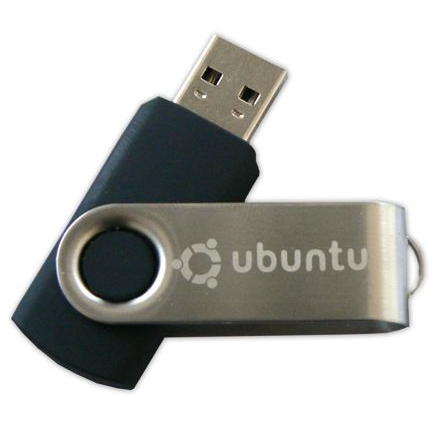
\includegraphics[width=0.5\textwidth]{flashboot}
  \caption{حافظه usb دارای ایمیج ابونتو و اماده بوت شدن توسط بایوس~\cite{usb_bootable}}
\end{figure}
\end{frame}

% صفحه ۵
\subsection{نصب از طریق شبکه}
\begin{frame}{نصب از طریق شبکه}
  خیلی از BIOS‌ها این اجازه را می‌دهنند که مراحل بوت شدن مستقیما با دانلود هسته و یک ایمیج خیلی کوچک از فایل سیستم‌ از طریق شبکه صورت گیرد.
  این متد نام‌های مختلفی دارد برای مثال PXE یا بوت TFTP و زمانی که شما دسترسی به CD-ROM یا درگاه USB ندارید شاید تنها راه شما باشد و کمک بسیار زیادی می‌کند.\\
\end{frame}
\note{
  در این متد مراحل نصب به دو قسمت تقسیم می‌شود.
اول، زمانی که رایانه در حال بوت شدن است بایوس(یا کارت شبکه) درخواست یک آدرس ای پی به طور خودکار می‌دهد.
بعد از اینکه سرور DHCP و BOOTP پاسخی دادند، پاسخ شامل filename و همچنین تنظیمات شبکه است.
بعد از تنظیمات شبکه، کامپیوتر کاربر برای یک فایل که نامش در درخواست قبلی بود(filename) درخواست  (Trivial File Transfer Protocol) TFTP ارسال می‌کند.
به محض رسیدن فایل،  به عنوان یک بوت-لودر اجرا می‌شود و سپس برنامه نصاب دبیین اجرا می‌شود و مراحل همانند مراحل قبل همانطور که بر روی CD یا USB storage بود، پیش می‌رود.
}

% صفحه ۶
\subsection{دیگر متدها}
\begin{frame}{دیگر متدهای نصب}
  وقتی بخواهیم دبیین یا هر توزیعی را در اسکیل گسترده‌ای و برای تعداد زیادی از رایانه‌ها نصب کنیم  معمولا از روش‌ها خودکار به جای روش دستی استفاده می‌کنیم.
به این صورت که با توجه به موقعیت و حساسیت‌ها و رایانه‌هایی که وجود دارند با یک نصاب شخصی سازی شده از روش FAI (Fully Automatic Installer) یا نصب تمام خودکار استفاده می‌شود.
\end{frame}

% صفحه ۷

\section{قدم به قدم با نصب آسان}
\subsection{بوت کردن و شروع نصب}
\begin{frame}{بوت کردن و شروع نصب}
  به محض بوت شدن CD یا DVD-ROM توسط بایوس، بوت-لودر فایل ایزو لینوکس نمایش داده می‌شود.\\
  در این مرحله هنوز هسته لینوکس بارگذاری نشده است، در منو به شما اجازه می‌دهد تا هسته را برای بوت انتخاب کنید و پارامترهای لازم برای طی روند بوت انتقال دهد.\\
  برای نصب استاندارد و آسان گزینه «install» یا «Graphical install» را انتخاب کنید(با استفاده کلید‌های اشاره). سپس دکمه «Enter» را فشار دهید تا روند مراحل نصب آغاز شود.\\
  اگر CPU سیستم inter یا AMD ۶۴ بیتی باشد در آن منو گزینه نصب ۶۴ بینی نیز فعال می‌شود همچنان که گزینه ۳۲ بیتی در یک زیر منو دیگر فعال است.\\
  اما اگر CPU سیستم فقط ۳۲ بیتی باشد در منو شما نمی‌توانید گزینه‌ای انتخاب کنید و ۳۲ بیتی نصب می‌شود.\\
\begin{figure}
    \centering
    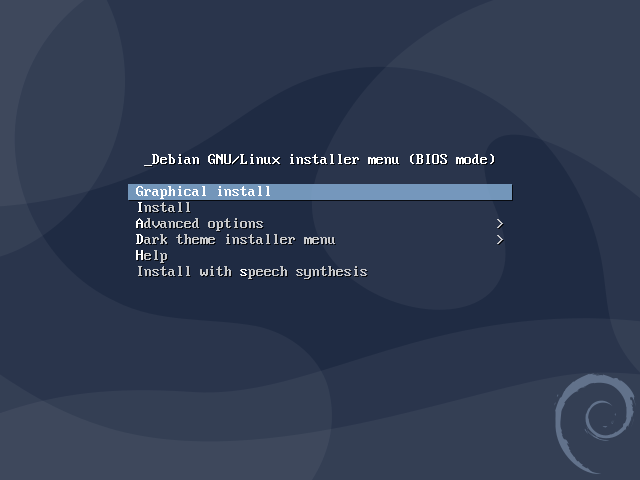
\includegraphics[width=0.5\textwidth]{bootloader}
    \caption{صفحه بوت~\cite{deb_bootscreen}}
\end{figure}
\end{frame}
\note{
  فرق ۳۲ بیتی و ۶۴ بیتی: فرق بنیانی یا اصلی این دو معماری در سایز مموری است. به طور تئوریک معماری ۳۲ بیتی نمی‌تواند با بیشتر از ۴ گیگ رم کار کند.

  مولتی بوت: اگر در راینه در حال حاضر ویندوز نصب است لازم به حذف آن نیست و امکان استفاده هر دوی آنها در یک دیسک وجود دارد و فقط لازم است دیسک را با توجه به نیاز هر کدام از سیستم عامل‌ها پارتیشن‌بندی کرد، و در موقع بوت شدن رایانه هر کدام را که خواستید انتخاب کنید.
  به این نوع پیکربندی اصطلاحا «dual boot» می‌گویند.

  بوت-لودر: یک برنامه سطح پایین است پس از بوت شدن رایانه توسط BIOS، بوت-لودر کرنل لینوکس رو بارگذاری می‌کند.
}

% صفحه ۸

\subsection{انتخاب زبان}
\begin{frame}{انتخاب زبان}
  شروع نصب در ابتدا با زبان انگلیسی است اما در مرحله انتخاب زبان با انتخاب زبان دیگر ادامه مراحل با زبان جدید نمایش داده می‌شود.\\
  \begin{figure}
    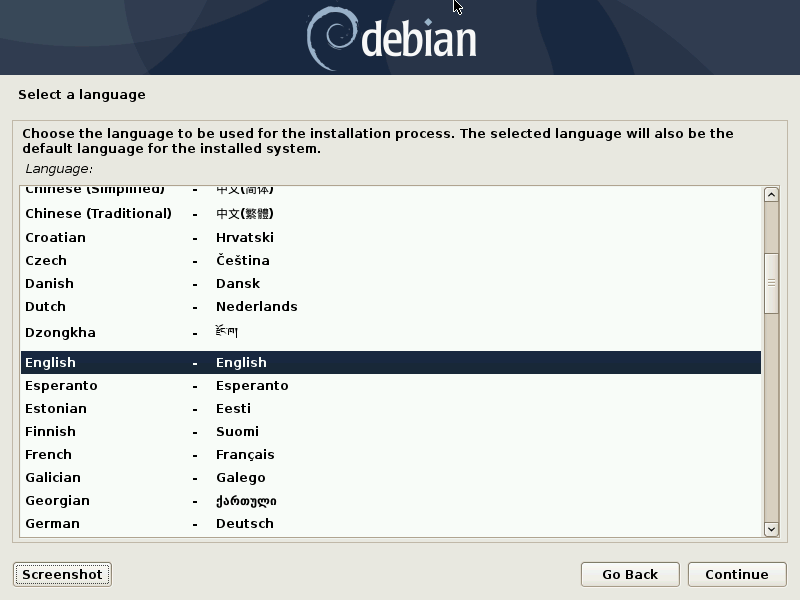
\includegraphics[width=.4\textwidth]{lang}
    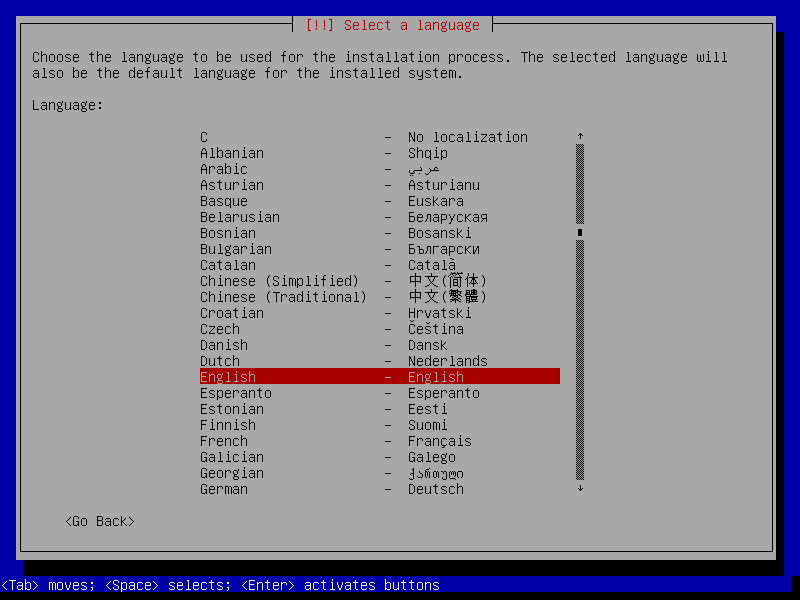
\includegraphics[width=.4\textwidth]{lang-cli}
    \caption{انتخاب زبان در محیط گرافیکی و متنی~\cite{deb_lang_gui}}
  \end{figure}
\end{frame}
\note{
  بعضی از مراحل نصب نیازمند ورود اطلاعات است،‌ در محیط متنی با استفاده دکمه Tab می‌توانید بین گزینه‌ها جابه‌جا شوید همچنین می‌توانید از کلید‌های اشاره نیز استفاده کنید.
  اما در محیط گرافیکی با استفاده از موس نیز میتوانید گزینه‌های خود را انتخاب کنید.
}

% صفحه ۹
\subsection{انتخاب کشور}
\begin{frame}{انتخاب کشور}
  مرحله بعدی انتخاب کشور است، این مرحله با ترکیب مرحله قبل که انتخاب زبان بود؛ مناسب‌ترین ساختار کیبود(keyboard layout) را برای شما انتخاب می‌کند.\\
  همچنین این مرحله موقعیت زمانی و مکانی (time zone) را در سیستم شما تنظیم می‌کند.\\
  در مرحله بعد نیز ساختار کیبور را به توجه به ساختاری که در کشورتان استفاده می‌شود انتخاب می‌کنید.
  \begin{figure}
    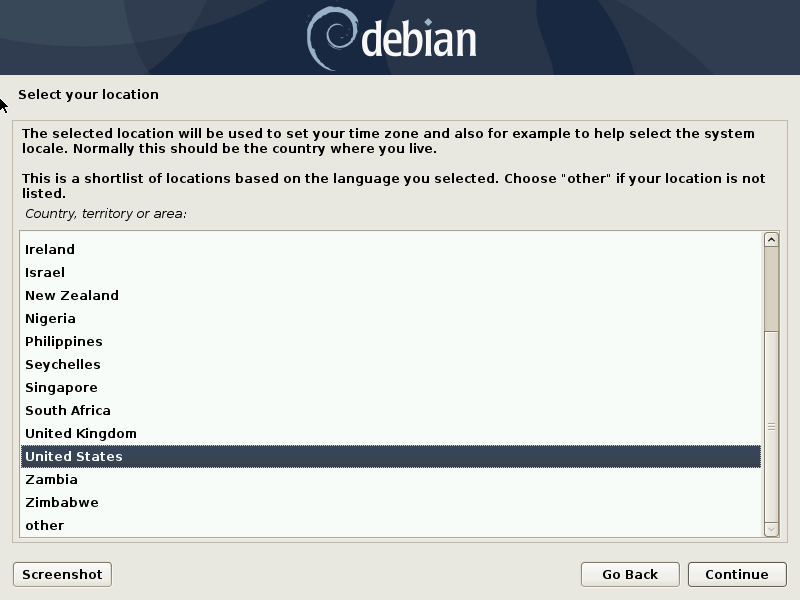
\includegraphics[width=.4\textwidth]{country-gui}
    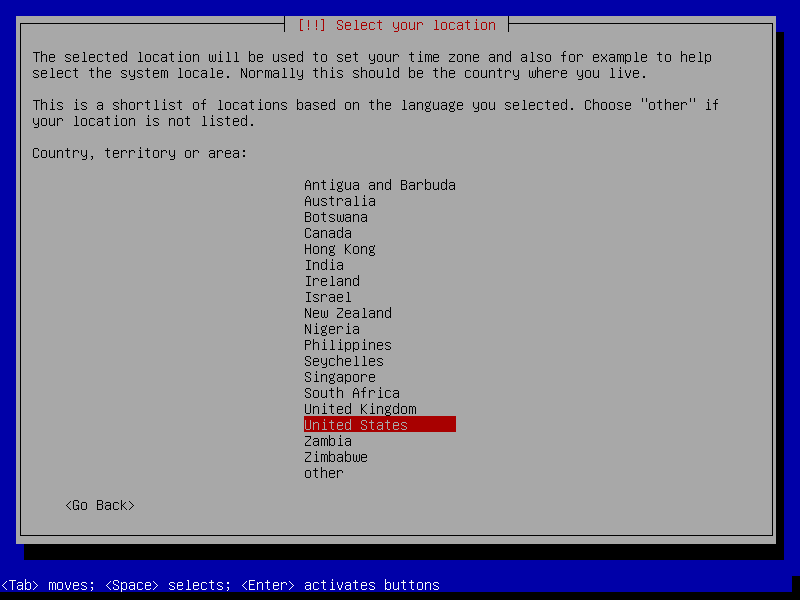
\includegraphics[width=.4\textwidth]{country-cli}
    \caption{انتخاب کشور در محیط گرافیکی و متنی~\cite{deb_country_gui}}
  \end{figure}
\end{frame}

% صفحه ۱۰

\subsection{شناسایی سخت افزار}
\begin{frame}{شناسایی شخت افزار}
  در این مرحله کارها به طور خودکار انجام می‌شوند. نصاب سخت افزارهای شما را تشخیص می‌دهد و سعی می‌کند تا برای دسترسی به محتوای CD یا حافظه USB آن‌ها را تشخیص دهد.\\
تمام مراحل قبلی تماماً در فایل ایمیج روی سی‌دی اتفاق افتادند. این فایل فایلی با حجم محدود است که هنگام بوت از سی‌دی توسط بایوس به حافظه اصلی منتقل می‌شود.
\end{frame}

\subsection{شناسایی سخت افزار شبکه و پیکربندی + بارگذاری اجزا دیگر}
\begin{frame}

\end{frame}

\subsection{رمز عبور کاربر ادمین }
\begin{frame}

\end{frame}

\subsection{ساخت اولین کاربر}
\begin{frame}

\end{frame}

\subsection{شناسایی دیسک حافظه و دیگر سخت افزارها}
\begin{frame}

\end{frame}

\section{پارتیشن بندی}
\begin{frame}

\end{frame}

\subsection{پارتیشن بندی خودکار}
\begin{frame}

\end{frame}

\subsection{پارتیشن بندی دستی}
\begin{frame}

\end{frame}

\section{پیکربندی نهایی}
\subsection{نصب اولیه سیستم}
\begin{frame}

\end{frame}

\subsection{پیکربندی مدیر پکیج‌ها}
\begin{frame}

\end{frame}

\subsection{انتخاب پکیج‌های مورد نیاز برای نصب}
\begin{frame}

\end{frame}

\subsection{نصب گراب}
\begin{frame}

\end{frame}

\section{اولین بوت}
\begin{frame}

\end{frame}

\subsection{نصب نرم افزارهای اضافه}
\begin{frame}

\end{frame}

\subsection{نحوه به روزرسانی کل سیستم}
\begin{frame}

\end{frame}

\refs
\end{document}
